\documentclass[]{article}

%opening
\title{MLP Coursework 4}
\author{Eskil Joergensen}
\date{\today}

\usepackage[parfill]{parskip}
\usepackage{pgfgantt}
\usepackage{multicol}
\usepackage{multirow}
\usepackage{tablefootnote}
\usepackage{tikz}
\usepackage{pgfplots}
\newcommand*\rot{\rotatebox{90}}
\usepackage{graphicx}
\graphicspath{ {images/} }

\usepackage{amsmath}

\usepackage{booktabs}
\usepackage[font={small,it}]{caption}

\begin{document}

\maketitle

\section{Introduction}

Fully connected neural networks are trained at a relatively low computational cost, and they have been used in machine learning for quite some time. However, current state-of-the-art networks are all convolutional neural networks (CNNs) \cite{long2015fully}. The high performance is (typically) achieved as the kernels in the convolutional layers extract features from the input data via their spacial locality. A common use case is object recognition in images, but can also be used in other tasks such as natural language processing \cite{Collobert}. 

Preliminary work has been done on the same data set using a fully connected neural network. More details are presented in the Background section (\ref{background}) below. 

CNNs introduce a significantly larger number of weights and connections, compared to a fully connected network, which means the parameters of the network must be carefully tuned to ensure adequately successful training. 

This report presents a series of experiments set to investigate how some key components of a CNN affect it's overall performance during training. Furthermore, the (optimal) findings from each experiment are integrated into the network for the subsequent experiments, trying to improve the performance of the network as much as possible. The following aspects of the CNN are investigated:

\begin{itemize}
	
	\item How does the size of kernels and number of feature maps in the convolutional layers affect the training? Different sizes of kernels, and number of feature maps will likely impact the computational cost of the network, but could a potential performance improvement be justified by the additional cost?
	
	\item How does the choice of activation function impact the performance of the network? More specifically, how will combinations of learning rates and non-linear activation functions affect the training of the network? 
	
	\item What type, and magnitude, of regularization is needed to overcome over-fitting of the CNN? Without any normalization or regularization significant over-fitting will likely occur. How can the performance of the network be maintained, while simultaneously reduce the amount of over-fitting?
	
\end{itemize}

In addition to improving the overall performance of the training of the network, the experiments were guided by a goal of 70\% accuracy on the validation data set. As a result, the methodology and incremental improvements to the model were made on these grounds. 

\subsection{Background} \label{background}

Preliminary experiments have been conducted on the same data, using a fully connected neural network. The network was trained using a variety of activation functions, hidden layer depths and widths as well as learning rate scheduler. 

\subsubsection{Activation Functions}

Four activation functions were compared. The logistic sigmoid $f(x)=\frac{1}{1+e^{-x}}$, the hyperbolic tangent $f(x)=tanh(x)$ the rectified linear (ReLu) $f(x)=max(0,x)$ and the exponential linear unit (ELU):

\begin{equation} \label{eq:elu}
f(x) = \begin{cases}
x &\text{if $x >$ 0}\\ \alpha (\text{exp}(x) - 1) &\text{if  $x \leq$ 0}
\end{cases}
\end{equation}

where \(\alpha\) is a hyperparameter that decides the range of negative values for which the activation function saturates.

The results showed that the ELU activation function outperformed the other three, with a final training and validation set accuracy of 66.9 \% and 50.5\% respectively. 

\subsubsection{Hidden layers}

Besides the one outsider, the training data shows a very similar performance for remaining five configurations. The two best trials were both from the models with three hidden layers.

\subsubsection{Learning Rate Schedule}

The results show that the training with the initial learning rate of 0.025 and 0.05 performed significantly better than the other initial learning rates (besides 0.02 and 0.03). As the error increases for learning rates lower than 0.025, as well as for learning rates over 0.05, it seems plausible that the optimal initial learning rate lies between 0.025 and 0.05 for the current model. 


\section{Methodology}


\subsection{The Network Architecture}

A neural network with two convolutional and two fully connected hidden layers was chosen for this study. The network also had two max pooling layers, one after each convolutional layer, as well as a 10-way softmax output classification. 

A model with only two convolutional layers were chosen due to time and computational resources available. Two convolutional layers allowed for observation of the added performance, while not making the network exceedingly costly to train. 

\begin{figure}[h]
	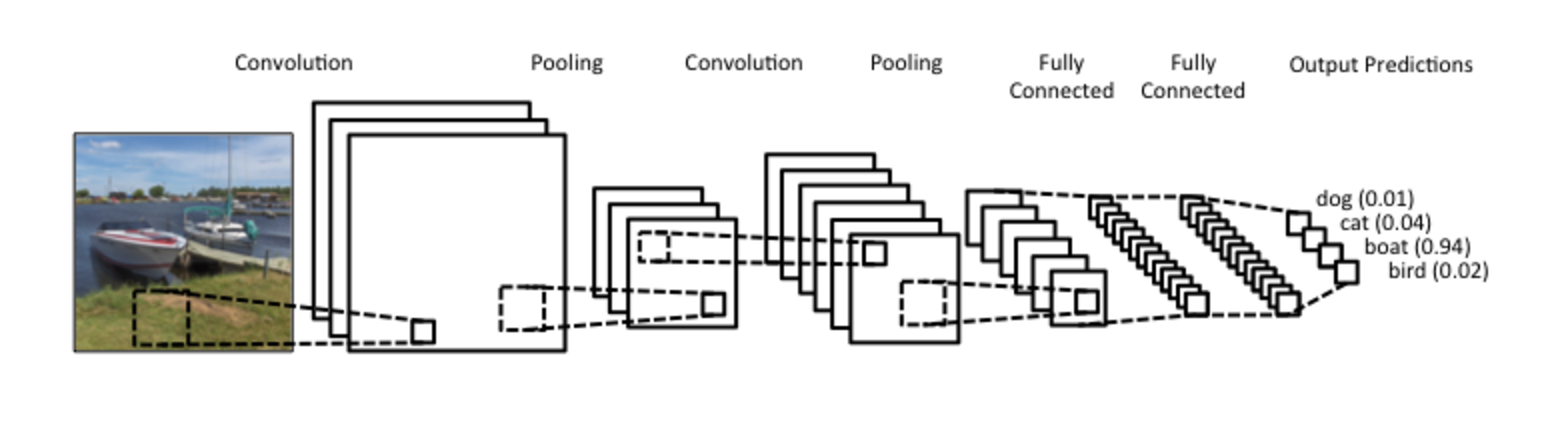
\includegraphics[width=\textwidth]{conv}
	\caption{Showing a visual representation of the convolutional neural network used.}
	\label{conv}
	\centering
\end{figure}

\subsubsection{Convolutional Layer}

The convolution in the convolutional layer was implemented using the \texttt{tf.nn.conv2d} method from TensorFlow (\texttt{tf}) with stride of 1 and no padding (\texttt{padding='SAME'}). The convolution operation was executed on the layer inputs together with the kernels (using the specified stride and padding). Both the layer inputs and the kernels were TensorFlow tensors, and the result of the convolutional operation was also a TensorFlow tensor. 

The biases were added to the tensor after the convolution. In the convolutional layers where batch normalization was specified, the tensor was normalized immediately after the biases were added to the convolutional tensor. Finally, an activation function was applied to the tensor, before passing the output on to the next layer. 

A truncated normal distribution was use to initialize the kernels, and the biases were initialized to zero. See Section \ref{weights}, Weight and Biases, for the specific implementation in TensorFlow. 

\subsubsection{Fully Connected and Output prediction Layer}

The fully connected and the classification output layers were implemented using the same class, as only a few factors separate the behavior of the two. A constant halving of the number of hidden units were integrated into all the fully connected layers, except the output prediction layer which had a 10-way output.

The weights and biases were initialized in the same as mentioned for the convolutional layers, only the weights for the affine layers were two dimensional. 

Finally, the inputs were multiplied with the weights using \texttt{tf.matmul} ,before the biases were added to the tensor. For the final classification layer this tensor would be returned, otherwise an activation function would be applied before returning the tensor.

\subsubsection{Pooling Layer}

The max pooling layer was implemented using the \texttt{tf.nn.max\_pool} method from TensorFlow. Each pooling layer used a 3 by 3 window for the sampling, and a stride of 2. Similarly to the convolutional layer the pooling layer used no padding, \texttt{padding='SAME'} in TensorFlow. 

\begin{figure}[h]
	\centering
	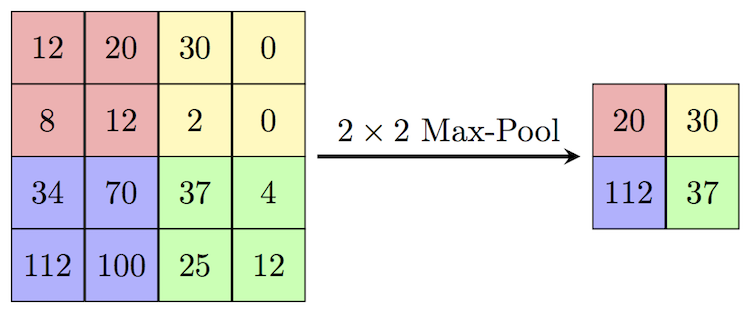
\includegraphics[width=0.6\textwidth]{pool}
	\caption{Showing an example of a 2x2 max pool operation. The 3x3 equivalent operation was used throughout this investigation.}
	\label{pool}
	\centering
\end{figure}

\subsubsection{Dropout Layer}

The dropout layer was implemented using \texttt{tf.nn.dropout(inputs, keep\_prop)}, and will keep each element in the input tensor with a probability of \texttt{keep\_prob}. 

\subsubsection{Batch Normalization}

The batch normalization of the convolutional layer was achieved with the \texttt{tf.nn.max\_pool} method from TensorFlow. Batch normalization transforms its input to zero mean and unit variance. By statistical analysis the batch normalization normalizes the inputs of a transformation layer. Equation \ref{batch_eq} shows how the inputs \(x_i\) are normalized

\begin{equation} \label{batch_eq}
BN(x_i) = \gamma_i \Big( \frac{x_i - \mu_i}{\sqrt{\sigma_i^2 + \epsilon}} \Big) + \beta_i
\end{equation}

where \(\mu_i\) is the batch mean, \(\sigma_i^2\) is the batch variance, \(\gamma_i\) is a scale factor and \(\beta_i\) is a shift factor. \(\gamma_i\) was set to 1.0, \(\beta_i\) to zero and \(\epsilon\) to 1e-3. The batch mean and variance was obtained from the inputs using \texttt{tf.nn.moments}. 


\subsubsection{Weights and Biases} \label{weights}

The weights used in both the convolutional and fully connected layers were initialized using a truncated normal distribution. The values were distributed with zero mean and a standard deviation of 0.1. Values more than two standard deviations away from the mean were dropped. The distributions were initialized with the \texttt{tf.truncated\_normal} method. 

The biases used were all initialized to zero using the \texttt{tf.zeros} method. Additionally, the weights and biases were added to the TensorFlow graph using  \texttt{tf.Variable}.

\subsection{Experimental Procedure}

The procedure used to tune the performance of the network involved three stages. During the initial stage the network was trained for few epochs, with a coarse spread of hyper parameter and multiple algorithms were tested during this phase. The overall results from the initial trials informed the finer range of parameters used for additional training and further tuning of hyper parameters. The second stage involved longer training. The third stage, before the final testing, the model was trained for significantly longer, and only a couple varieties of the model were used. 

The default baseline model used has two convolutional layers, two fully-connected layers and finally a softmax classification layer. The network also had two 2x2 pooling layers after each convolutional layer. 

\subsubsection{Activation Functions}

The model was trained using three learning rates, with the four activation functions used in the preliminary experiments: ReLu, Elu, Tahn and Sigmoid. During the first round of trials the network was trained for 5 epochs. A relatively large, non-uniform spread of the learning rate was chosen intentionally to observe how the activation functions would react to the different rates. 

After the initial trials, the best two activation functions were kept for further experimentation, and the other two were discarded. The learning rates were also narrowed down, closer to the best performing learning rate. All activation functions, learning rates and training epochs used during the investigation can be seen in Table \ref{ac-overview}.

Again, after the second round, the learning rates were modified before the last round of training. As the two last activation functions performed similarly, both were tested in the final trials. The combination of learning rate and activation functions, that resulted in best performance, was then used for the during the next set of experiments, see Section \ref{filter-methods}.

\begin{table}[h]
	\centering
	\caption{Showing the combinations of activation functions, learning rates and training duration in Epochs, for the three rounds of experimentation.}
	\label{ac-overview}
	\begin{tabular}{@{}cccc@{}}
		\toprule
		Round & Learning Rates & Activation Fn. & Training Epochs \\ \midrule
		1 & 5e-4, 3e-3, 0.01 & ReLu, Elu, Tanh, Sigmoid & 5 \\
		2 & 1e-4, 9e-4 & ReLu, Elu & 10 \\
		3 & 4e-4, 7e-4 & ReLu, Elu & 15 \\ \bottomrule
	\end{tabular}
\end{table}

The effect of the learning rates and non-linear activation functions on the aforementioned network were tested with 3x3 kernels and 24 feature maps. The network did not use any kind of L2 regularization, batch normalization or drop out. 

The procedure used to train the network is presented in Section .

\subsubsection{Filter Sizes and Feature Maps} \label{filter-methods} 

During the second part of the experimentation, the network was trained with nine combinations of kernel sizes and feature maps. The size of kernels were 3, 5 and 7, whereas the number of feature maps were 16, 24 and 32. During the first round the network was trained for 5 epoch, using the ELU activation function was used with a learning rate of 0.0004. 

The network was supposed to be trained in three rounds, incrementally determining the best combination of kernel size and number of feature maps. However, due to exceedingly long training times and swap memory warnings (during the two most expensive trials) the two later rounds were not completed. 

The three combinations with 32 feature maps all performed similarly, but at very different completion times and computational cost. See Table \ref{filter-res} for execution times. The 3x3 kernel and 32 feature maps were used for the remaining experimentation. 

\subsubsection{Regularization and Normalization}

As with the previous experiments, short first round trials were run using coarse set of parameters. The network was trained using eight different combinations of batch normalization, drop out and L2 weight decay. The regularization and normalization parameters used in all three rounds can be seen in Table \ref{reg-table}. The batch normalization only applied to the convolutional layers and the dropout 

Using three nested loops, the network was trained using eight different combinations of batch normalization, drop out and L2 weight decay. The batch normalization added to the convolutional layers were either true or false, the L2 decay was none or 0.0005 and the keep probability of the dropout layers were either 1.0 (keep all) or 0.5. The network was trained for 5 epochs during the first set of trials. 

The third round of training used 20 epochs instead of 15, as the regularization slowed down the training.

\begin{table}[h]
	\centering
	\caption{Showing the combinations of parameters used during the normalization and regularization investigative rounds.}
	\label{reg-table}
	\begin{tabular}{@{}ccccc@{}}
		\toprule
		Round & Batch Norm. & Dropout Prob. & L2 Reg. & Training Epochs \\ \midrule
		1 & True, False & None, 0.5 & None, 5e-4 & 5 \\
		2 & True & 0.45, 0.55 & 5e-4 & 10 \\
		3 & True & 0.5 & 5e-4, None & 20 \\ \bottomrule
	\end{tabular}
\end{table}

The training runs were done with 3x3 kernels and 32 feature maps in each of the convolutional layers. 

\subsection{Network Training and Data Collection}

The TensorFlow graph was built using data placeholder of batch size 50. The progress of the training was visualized using TensorBoard, a visualization feature of TensorFlow. The batch normalized training data was also written to disk using numpy's savez. 

During training, the validation set was evaluated every 100 steps, as well as the first as last step. The validation set was not evaluated every step due to the significant computational cost that incurs. 

The network prediction output was determined using the \texttt{tf.softmax\_cross\_entropy\_with\_logits} from TensorFlow.  This also meant the softmax could be omitted in the final affine layer in the network. This investigation did not make use of a explicit learning rate scheduler, but the 'self-tuning' Adam Optimizer, \texttt{tf.train.AdamOptimizer} in TensorFlow, was used. The optimizer was used with varying learning rates, but with beta1=0.9, beta2=0.999 and epsilon = 1e-8 (default parameters) throughout the investigation. 
 
\section{Results}

All tests were performed on a macOS Sierra 10.12. operating system, with an Intel i5 2.6 GHz processor and 8 GB DDR3 memory with 1600 MHz. All trials were executed inside a custom mlp Python 2.7 virtual environment. 

\subsection{Activation Functions}

Training the network with the linear unit activation functions, ReLu and ELU, resulted in the stronger overall performance compared to the training outcome with the sigmoid or hyperbolic tangent. 

\begin{table}[h]
	\centering
	\caption{Showing the final validation classification accuracy  for the four activation functions, after 5 epochs, for different learning rates. The classification accuracies are reported as percentages.}
	\label{ac-table}
	\begin{tabular}{@{}c|cccc@{}}
		\toprule
		Learning Rate & ELU & ReLu & Tanh & Sigmoid \\ \midrule
		5e-4 & 69.5 & 70.27 & 67.7 & 46.9 \\
		3e-3 & 62.2 & 61.3 & 10.0 & 10.0 \\
		0.01 & 10.0 & 10.0 & 10.0 & 10.0 \\ \bottomrule
	\end{tabular}
\end{table}

The lowest learning rate, 0.0005, resulted in the highest classification accuracies across all the activation functions, and the ReLu trial had a final validation accuracy of 70.3\%. Training the network with a learning rate of 0.01 resulted in high total error and very low accuracies. In a 10-way classification task, 10\% accuracy means the final output are guesses, and no (useful) learning has occurred.

The training of the network during the final two rounds resulted in comparable final error and classification accuracies, see Figure \ref{ac_res}. The highest validation accuracy was 71.6\%, by ELU with the learning rate of 0.0004, and the lowest was 69.7\% by ReLu with the learning rate of 0.0007. Although the validation accuracy was over 70\%, the training set accuracies were much higher, which indicates a high degree of over-fitting. The over-fitting was also reflected in the validation set errors.

\begin{figure}[h]
	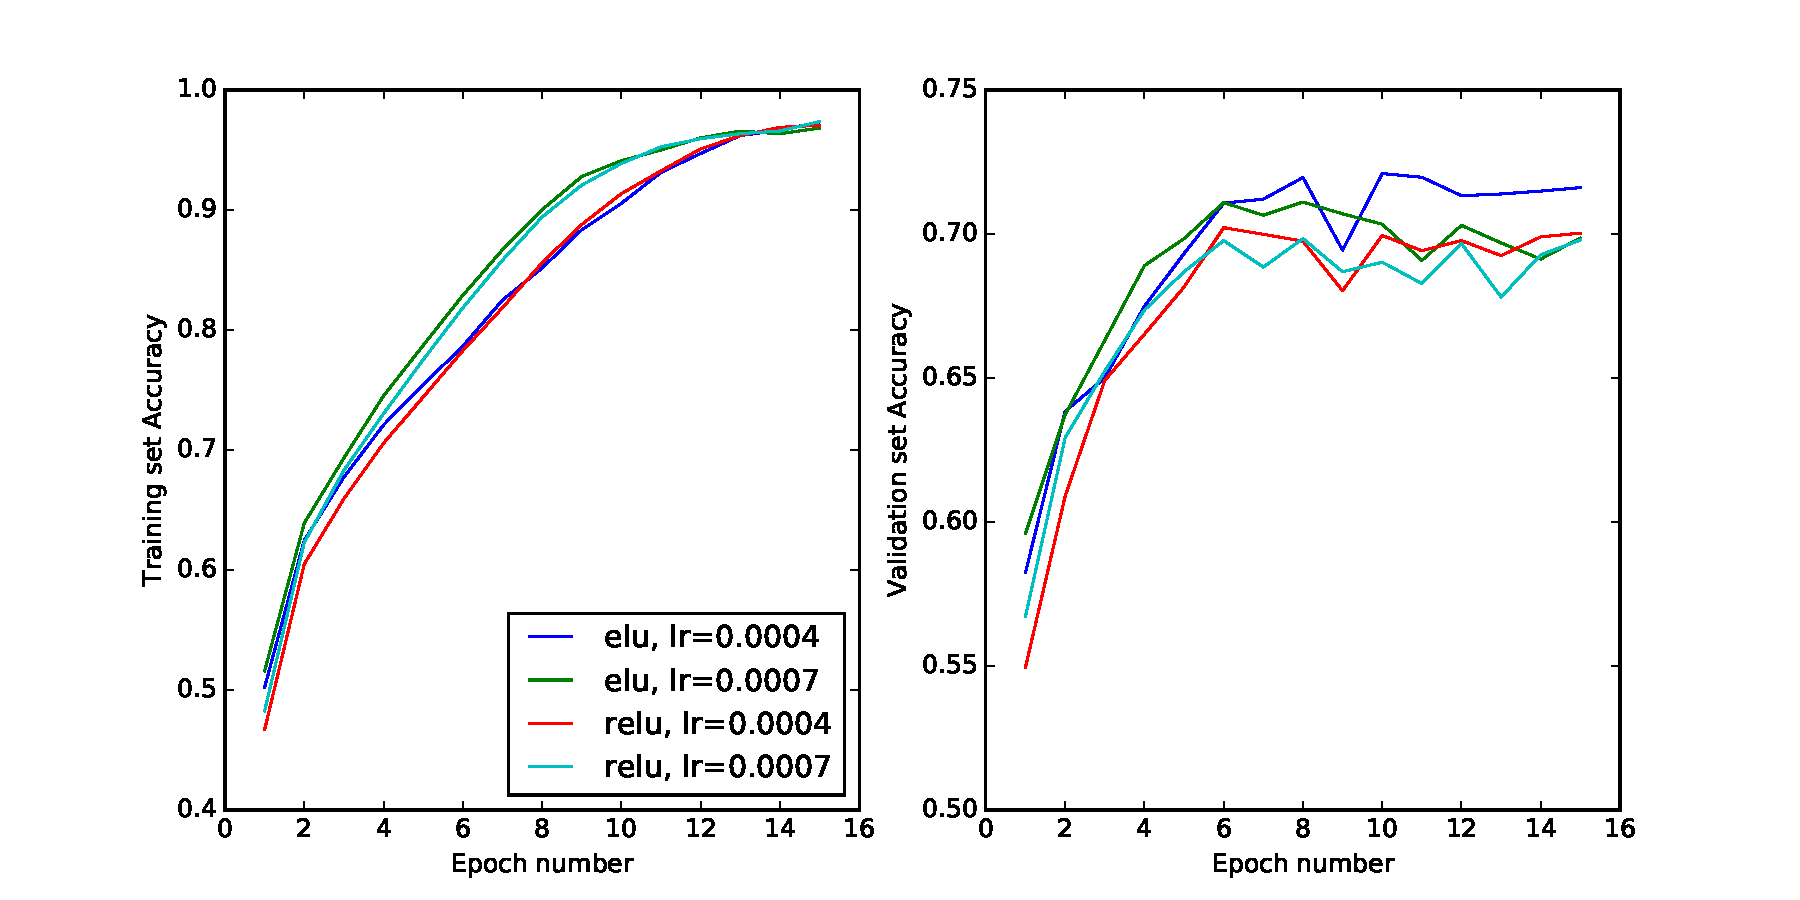
\includegraphics[width=\textwidth]{ac_res}
	\caption{Showing a visual representation of the model used, from TensorBoard.}
	\label{ac_res}
	\centering
\end{figure}

Compared to the training of the fully connected network, presented in Section \ref{background}, the choice of the activation functions effect the training performance of the CNN and the fully connected network in similar way. 

\subsection{Filter Sizes and Feature Maps}

The number of feature maps had a greater impact on the training performance, compared to the size of the kernels. As shown in Figure \ref{kernel_res}, the three best performing trials were all using convolutional layers with 32 feature maps. 

\begin{figure}[h]
	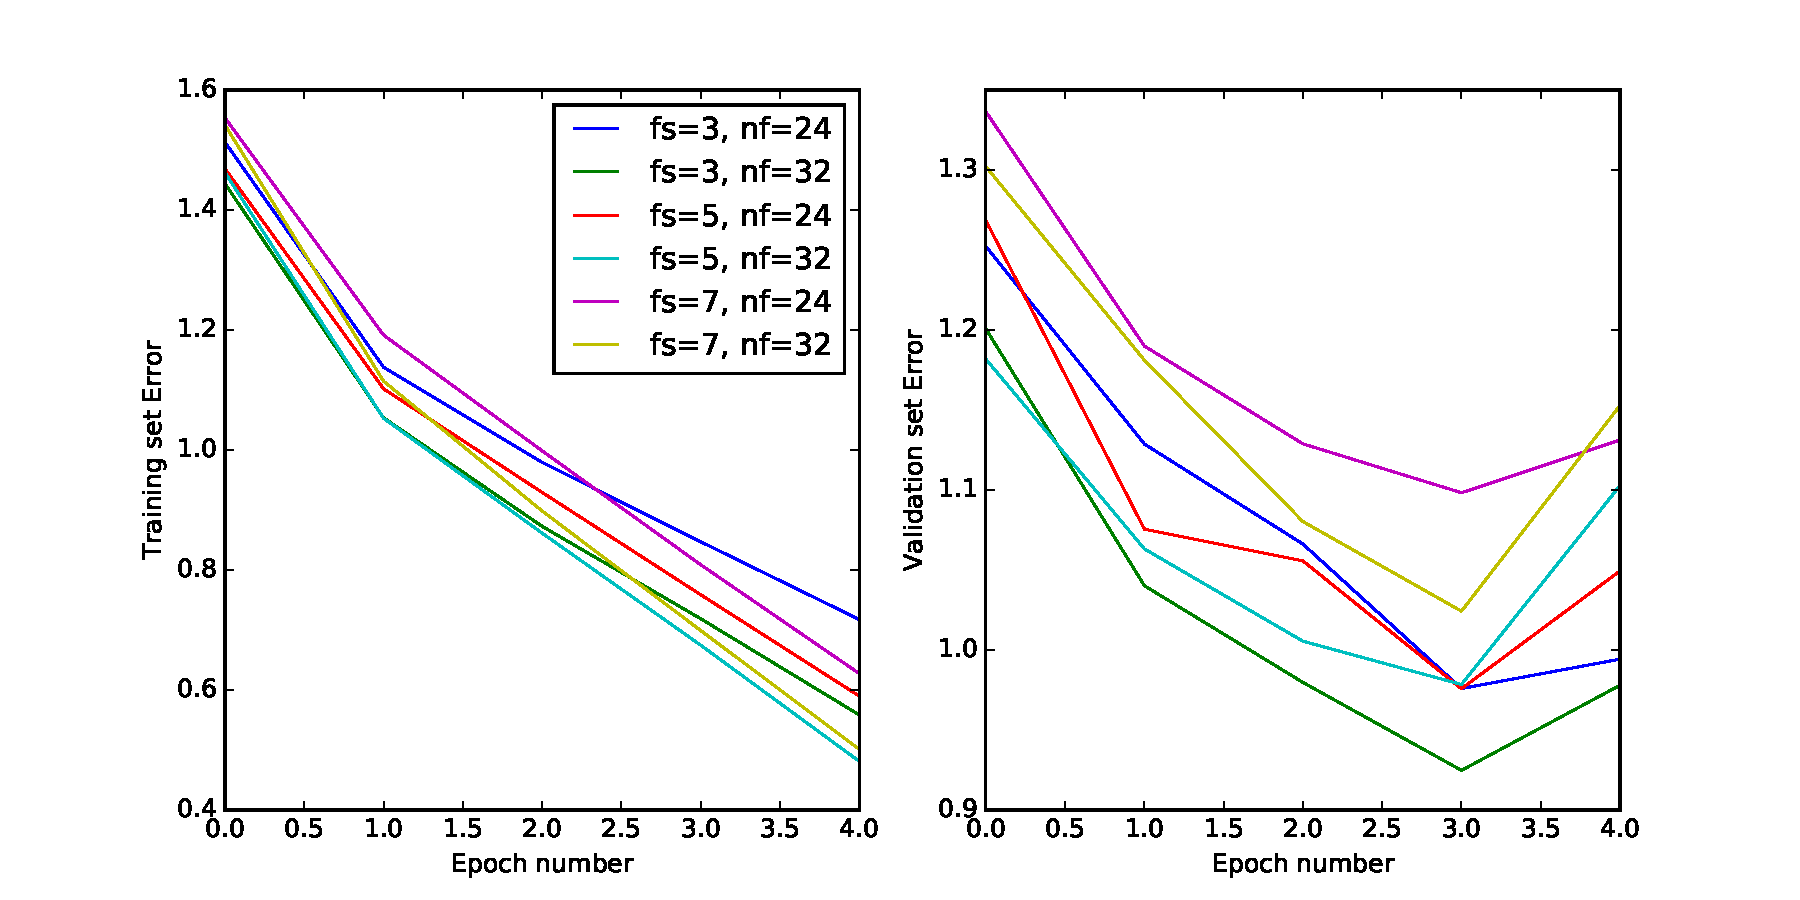
\includegraphics[width=\textwidth]{kernel_res}
	\caption{Showing the training and validation set errors for different kernel sizes and number of feature maps in each convolutional layer. fs = 'Filter Size', nf = 'number of filters'. }
	\label{kernel_res}
	\centering
\end{figure}

In contrast to the similar performance of the networks with 32 feature maps, the computational cost were sizable larger when trained using larger kernels. With a 10.7\% improvement in training set error, the CNN with the 7x7 kernel needed more than twice the execution time of the 3x3 CNN.

\begin{table}[h]
	\centering
	\caption{Showing the training execution time, in minutes, for 5 epochs for different kernel sizes and number of feature maps in the convolutional layers.}
	\label{filter-res}
	\begin{tabular}{@{}ccccc@{}}
		\toprule
		\multicolumn{2}{c}{Feature Maps} & 16 & 24 & 32 \\ \midrule
		\multirow{3}{*}{\rot{Size}} & \multicolumn{1}{c|}{3x3} & 12.5 & 19.1 & 27.0 \\
		& \multicolumn{1}{c|}{5x5} & 22.5 & 34.6 & 49.1 \\
		& \multicolumn{1}{c|}{7x7} & 39.9 & 57.9 & 67.0 \\ \bottomrule
	\end{tabular}
\end{table}

Similarly to the study of the depth and width of the hidden layers in the fully connected neural network, additional hidden units, or connections, offer a small overall improvement in the training performance. The improvements come at a high computational cost, and are potentially only relevant to the state-of-the-art networks willing to sacrifice time and additional resources to achieve small performance improvements. 

\subsubsection{Regularization and Normalization}

The combination of batch normalization in the convolutional layers, L2 weight decay and 50\% dropout resulted in the greatest reduction of over-fitting, see Figure \ref{norm_diff}. Although the overall rate of training decreased, the gap between the training and validation set accuracies were reduced with each additional type of regularization. 

\begin{figure}[h]
	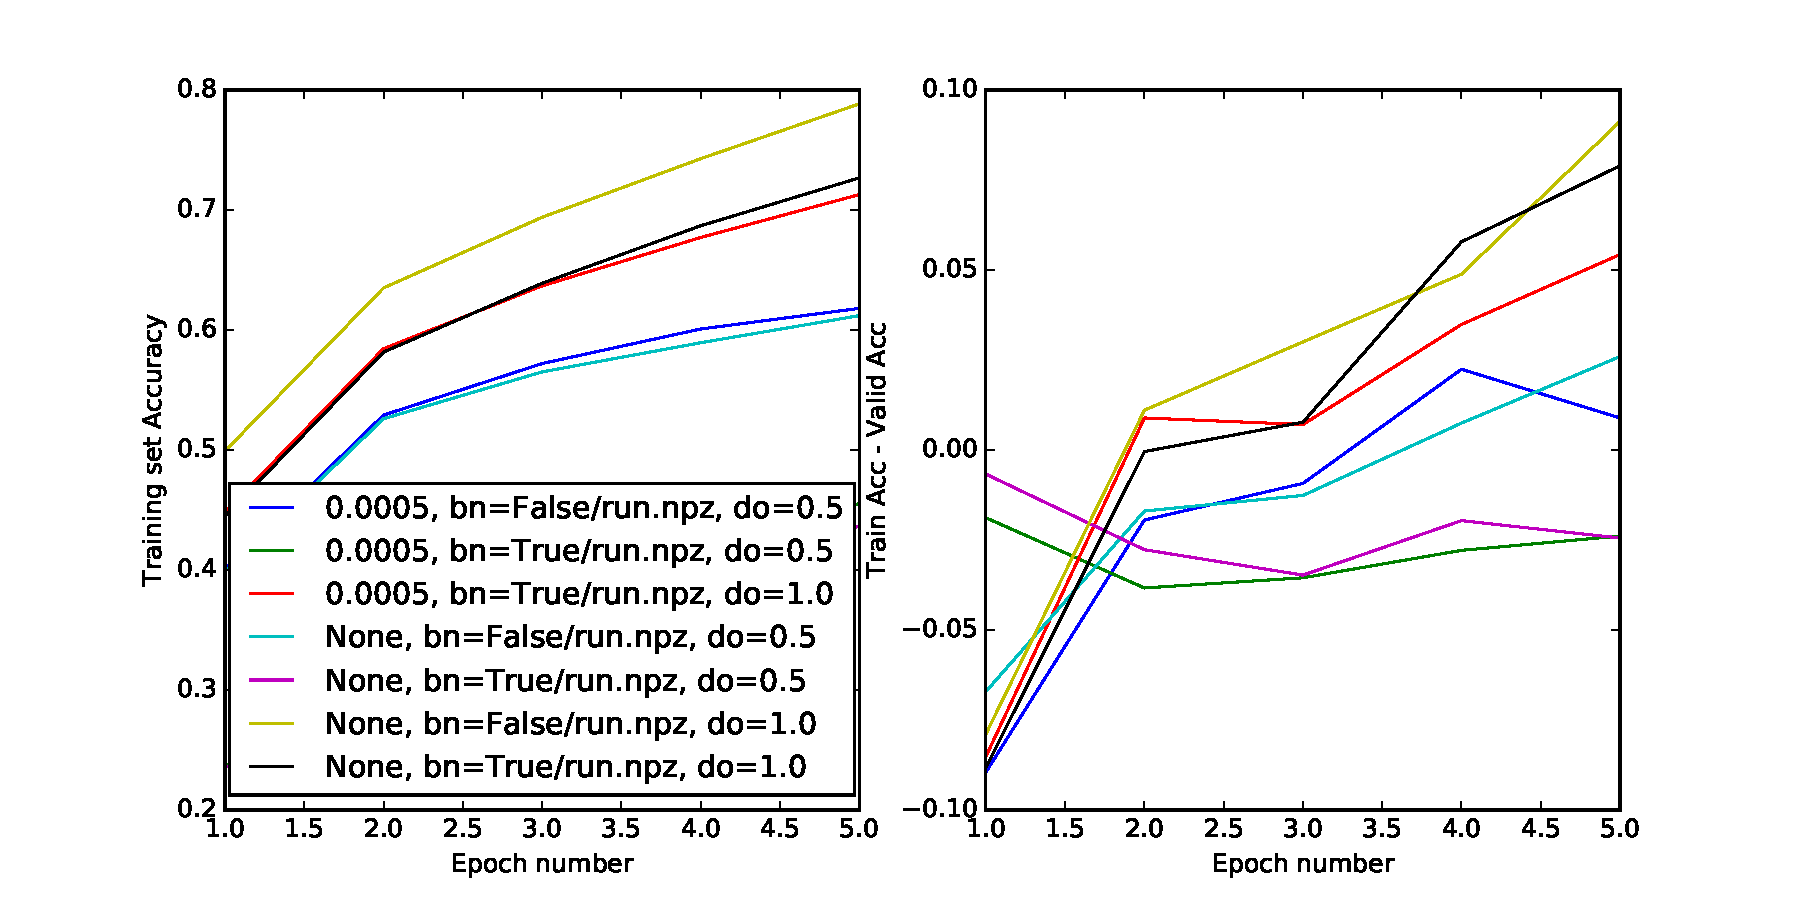
\includegraphics[width=\textwidth]{norm_diff}
	\caption{Showing the training set accuracy, and the difference between the traing and validation set accuracies for different normalization and regularization methods. } 
	\label{norm_diff}
	\centering
\end{figure}

Comparing the best performing trial from the Activation Functions Section, and the fully regularized and normalized network, the over-fitting is almost completely removed, see Figure \ref{before_after}. Even though the performance has not increased (when trained over similar number of epochs), the performance of the network could be improved further by repeating the optimization cycle shown in this report. Moreover, other forms of regularizations could be introduced to the training, such as data augmentation. 

\begin{figure}[h]
	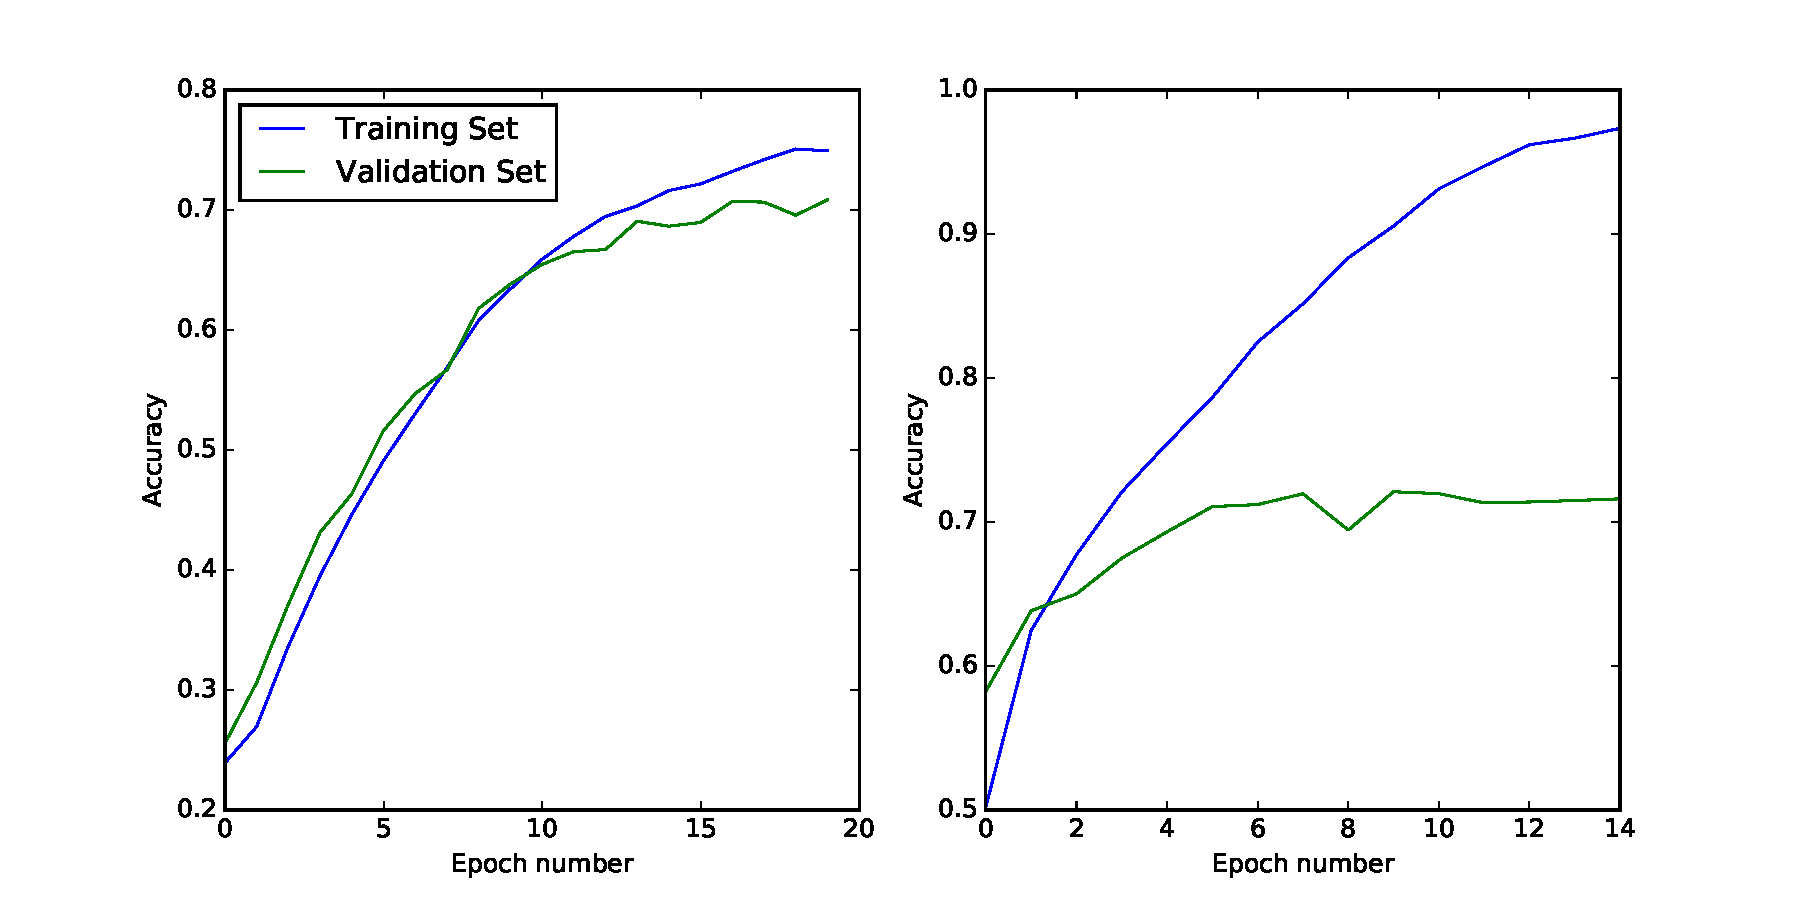
\includegraphics[width=\textwidth]{before_after}
	\caption{Showing the training and validation set accuracy of the regularized and normalized network on the left, and the non-normalized accuracies on the right. The plot on the right is the best performing trial from the first set of experiments. } 
	\label{before_after}
	\centering
\end{figure}

\section{Conclusion}

This report has presented a set of experiments, or a strategy, that can be used to improve the validity of a convolutional neural network. Through small iterations in parameter-space, and by introducing appropriate tools to reduce over-fitting, the overall performance of the network showed incremental improvements. 

Additional investigations could have gone into the use of data augmentation, as well as more advanced use of kernel sizes and feature maps in different convolutional layers. However, if the presented strategy for training optimization was applied to the network repeatedly, the performance would likely improve further. 

\clearpage
\medskip
\bibliographystyle{IEEEtran}
\bibliography{ref.bib}

\end{document}
